%%% LaTeX Template: Article/Thesis/etc. with colored headings and special fonts
%%%
%%% Source: http://www.howtotex.com/
%%% Feel free to distribute this template, but please keep to referal to http://www.howtotex.com/ here.
%%% February 2011
%%%
%%% Modified May 2018 by CDM

%%%  Preamble
\documentclass[11pt,letterpaper]{article}
\usepackage[margin=1.0in]{geometry}
\usepackage[T1]{fontenc}
\usepackage[bitstream-charter]{mathdesign}
\usepackage[latin1]{inputenc}					
\usepackage{amsmath}						
\usepackage{xcolor}
\usepackage{cite}
\usepackage{hyphenat}
\usepackage{graphicx}
\usepackage{float}
\usepackage{subfigure}
\usepackage{sectsty}
\usepackage[compact]{titlesec} 
\usepackage[tablegrid]{vhistory}
\allsectionsfont{\color{accentcolor}\scshape\selectfont}

%%% Definitions
\definecolor{accentcolor}{rgb}{0.0,0.0,0.5} 
\newcommand{\teamname}{Team Name}
\newcommand{\productname}{Product Name}
\newcommand{\coursename}{CSE 4316: Senior Design I}
\newcommand{\semester}{Spring 2018}
\newcommand{\docname}{System Requirements Specification}
\newcommand{\department}{Department of Computer Science \& Engineering}
\newcommand{\university}{The University of Texas at Arlington}
\newcommand{\authors}{Alan Turing \\ Grace Hopper \\ John Von Neumann \\ Ada Lovelace \\ Charles Babbage}

%%% Headers and footers
\usepackage{fancyhdr}
	\pagestyle{fancy}						% Enabling the custom headers/footers
\usepackage{lastpage}	
	% Header (empty)
	\lhead{}
	\chead{}
	\rhead{}
	% Footer
	\lfoot{\footnotesize \teamname \ - \semester}
	\cfoot{}
	\rfoot{\footnotesize page \thepage\ of \pageref{LastPage}}	% "Page 1 of 2"
	\renewcommand{\headrulewidth}{0.0pt}
	\renewcommand{\footrulewidth}{0.4pt}

%%% Change the abstract environment
\usepackage[runin]{abstract}			% runin option for a run-in title
%\setlength\absleftindent{30pt}			% left margin
%\setlength\absrightindent{30pt}		% right margin
\abslabeldelim{\quad}	
\setlength{\abstitleskip}{-10pt}
\renewcommand{\abstractname}{}
\renewcommand{\abstracttextfont}{\color{accentcolor} \small \slshape}	% slanted text

%%% Start of the document
\begin{document}

%%% Cover sheet
{\centering \huge \color{accentcolor} \sc \textbf{\department \\ \university} \par}
\vspace{1 in}
{\centering \huge \color{accentcolor} \sc \textbf{\docname \\ \coursename \\ \semester} \par}
\vspace{0.5 in}
\begin{figure}[h!]
	\centering
   	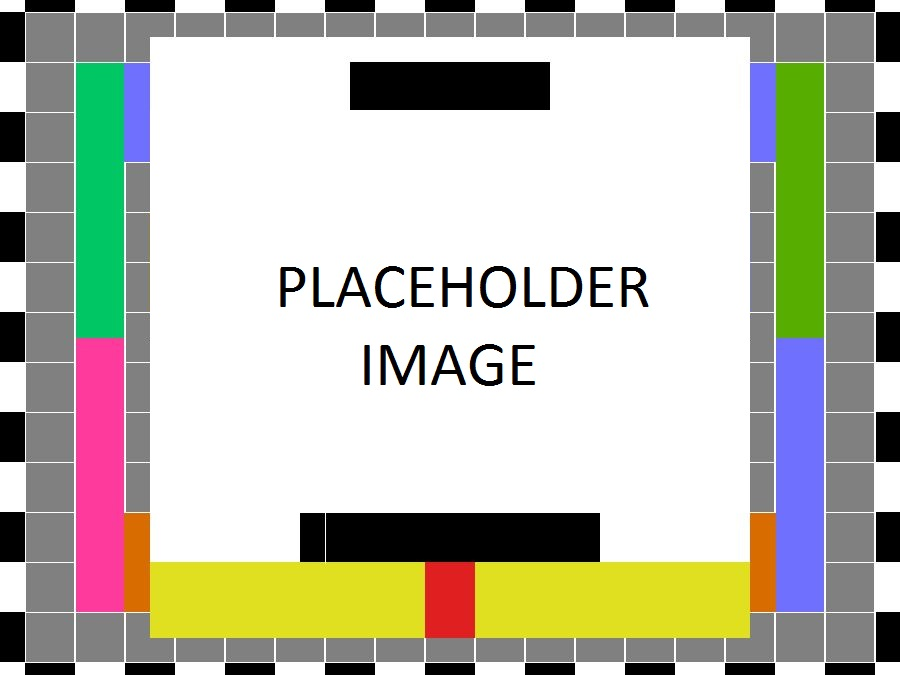
\includegraphics[width=0.60\textwidth]{images/test_image}
\end{figure}
\vspace{0.5 in}
{\centering \huge \color{accentcolor} \sc \textbf{\teamname \\ \productname} \par}
\vspace{0.5 in}
{\centering \large \sc \textbf{\authors} \par}
\newpage


%\vspace{1 in}
%\centerline{January 13th, 2012}
%\newpage

%%% Revision History
\begin{versionhistory}
  	\vhEntry{0.1}{10.01.2015}{GH}{document creation}
  	\vhEntry{0.2}{10.05.2015}{AT|GH}{complete draft}
  	\vhEntry{0.3}{10.12.2015}{AT|GH}{release candidate 1}
  	\vhEntry{1.0}{10.20.2015}{AT|GH|CB}{official release}
  	\vhEntry{1.1}{10.31.2015}{AL}{added customer change requests}
\end{versionhistory}
\newpage

%%% Table of contents
\setcounter{tocdepth}{3}
\tableofcontents
\newpage

%%% List of figures and tables (optional)
\listoffigures
%\listoftables
\newpage

\section{Product Concept}
This section provides a high-level statement of your product concept - what it is intended to do and how it is intended to be used. Include in this header paragraph, a brief synopsis of what is described here. For example, this header paragraph might say something like: "This section describes the purpose, use and intended user audience for the X product. X is a system that performs Y. Users of X will be able to Z..."

\subsection{Purpose and Use}
This is where you describe in a brief, yet clear and concise, manner what your product should do and how you expect it should be used.

\subsection{Intended Audience}
This is where you describe the intended audience(s) of your product. If this product were to be made available publicly or commercially, who would purchase or use it? Is the product designed for a particular customer, or an overall class of customers? Is it intended for general use, or is it a specific component of a more complex system?

\begin{figure}[h!]
	\centering
   	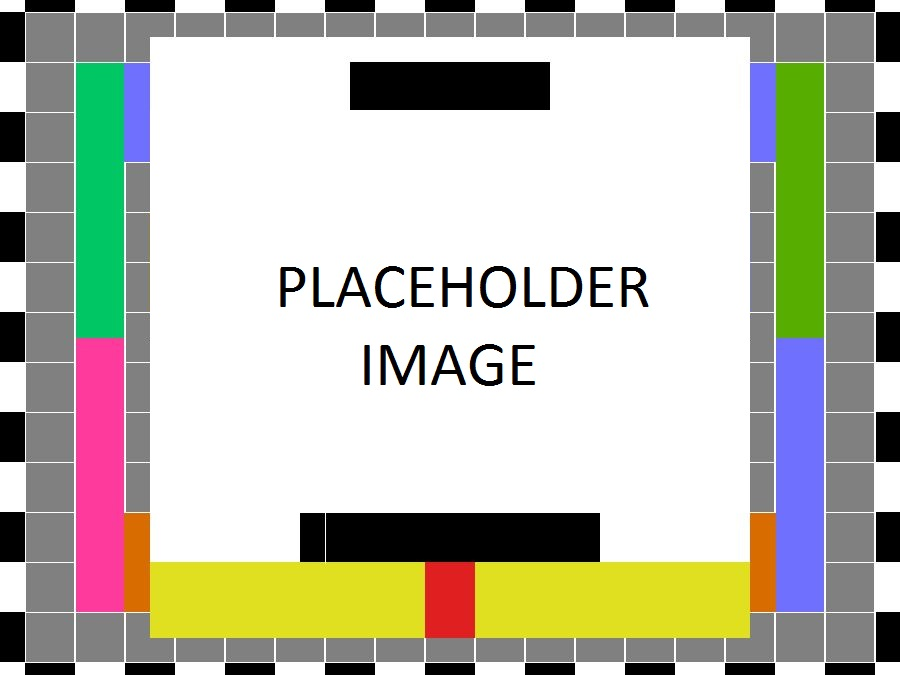
\includegraphics[width=0.60\textwidth]{images/test_image}
    \caption{X conceptual drawing}
\end{figure}

\newpage
\section{Product Description}
%This section provides a description of your product and defines it's primary features and functions. The purpose is to give the document reader/reviewer enough information about the product to allow them to easily follow the specification of requirements found in the remainder of the document. Your header for this section should introduce the section with a brief statement such as: "This section provides the reader with an overview of X. The primary operational aspects of the product, from the perspective of end users, maintainers and administrators, are defined here. The key features and functions found in the product, as well as critical user interactions and user interfaces are described in detail." Using words, and pictures or graphics where possible, specify the following:

This section provides a general overview of the Cerberus wrist module system. Described here are the features that our product provides, how our product interacts with its environment and user and how the interface will look for the Cerberus app and wrist module.
\subsection{Features \& Functions}
%What the product does and does not do. Specify in words what it looks like, referring to a conceptual diagram/graphic (Figure X).  Define the principle parts/components of the product. Specify the elements in the diagram/graphic that are part(s) of this product as well as any associated external elements (e.g., the Internet, an external web server, a GPS satellite, etc.)

The Cerberus system alerts wearers of events like their doorbell ringing, a door or window opening or noise around them. Figure 1 shows what happens when the doorbell ringing event occurs. The Cerberus system has hardware and software components. The wrist module notifies the wearer by vibrating on the wrist. The Cerberus app, which will be available for Android, identifies the event that caused the vibration via a notification. Users will create an account on the app to register their wrist module with their phone. In addition, the user can alter certain settings in the app to further control the wristband. The Cerberus server will store the user's account information like settings, username, password and phone number. The server will communicate externally with the Ring system, which the product will depend on for notifications. 

\subsection{External Inputs \& Outputs}
%Describe critical external data flows. What does your product require/expect to receive from end users or external systems (inputs), and what is expected to be created by your product for consumption by end users or external systems (outputs)? In other words, specify here all data/information to flow into and out of your systems. A table works best here, with rows for each critical data element, and columns for name, description and use.

\begin{table}[h]
\begin{tabular}{|l|l|l|}
\hline
Data Element & Input/Output & Description \\ \hline
Ring System notifications & Input & \begin{tabular}[c]{@{}l@{}}Notifications sent from the Ring System will be \\ intercepted by our server. These notifications will \\ be pushed to our phone app.\end{tabular} \\ \hline
App notifications & Output & \begin{tabular}[c]{@{}l@{}}The app will relay the notifications being sent \\ from the Ring system. The relays will come in\\ the form of notifications displayed to the user. \\ The relaying will also trigger the wrist module \\ vibration.\end{tabular} \\ \hline
Physical vibrations & Output & \begin{tabular}[c]{@{}l@{}}This will come from the wrist module. When \\ the Cerberus app receives a notification from \\ Ring, the wrist module will vibrate.\end{tabular} \\ \hline
\end{tabular}
\end{table}

\subsection{Product Interfaces}
%Specify what all operational (visible) interfaces look like to your end-user, administrator, maintainer, etc. Show sample/mocked-up screen shots, graphics of buttons, panels, etc. Refer to the critical external inputs and outputs described in the paragraph above.
Nothing to show yet.
\newpage
\section{Customer Requirements}
Include a header paragraph specific to your product here. Customer requirements are those required features and functions specified for and by the intended audience for this product. This section establishes, clearly and concisely, the "look and feel" of the product, what each potential end-user should expect the product do and/or not do. Each requirement specified in this section is associated with a specific customer need that will be satisfied. In general Customer Requirements are the directly observable features and functions of the product that will be encountered by its users. Requirements specified in this section are created with, and must not be changed without, specific agreement of the intended customer/user/sponsor.

\subsection{Requirement Name}
\subsubsection{Description}
A detailed description of the feature/function that satisfies the requirement. For example: \textit{The GUI background will be slate blue. This specific color is required in order to ensure that the GUI matches other similar software products offered by the customer. Slate blue is specified as \#007FFF, using six-digit hexadecimal color specification.} It is acceptable and advisable to include drawings/graphics in the description if it aids understanding of the requirement.
\subsubsection{Source}
The source of the requirement (e.g. customer, sponsor, specified team member (by name), federal regulation, local laws, CSE Senior Design project specifications, etc.)
\subsubsection{Constraints}
A detailed description of realistic constraints relevant to this requirement. Economic, environmental, social, political, ethical, health \& safety, manufacturability, and sustainability should be discussed as appropriate.
\subsubsection{Standards}
A detailed description of any specific standards that apply to this requirement (e.g. \textit{NSTM standard xx.xxx.x. color specifications \cite{Rubin2012}}. Standards exist for practically everything (ATC standard fuses, IEEE 802.15.4 embedded wireless, TLS 1.3 encryption, etc.), so be sure that you research and document which ones will be followed in meeting this requirement.
\subsubsection{Priority}
The priority of this requirement relative to other specified requirements. Use the following priorities:
\begin{itemize}
\item Critical (must have or product is a failure)
\item High (very important to customer acceptance, desirability)
\item Moderate (should have for proper product functionality);
\item Low (nice to have, will include if time/resource permits)
\item Future (not feasible in this version of the product, but should be considered for a future release).
\end{itemize}

\subsection{Requirement Name}
\subsubsection{Description}
Detailed requirement description...
\subsubsection{Source}
Source
\subsubsection{Constraints}
Detailed description of applicable constraints...
\subsubsection{Standards}
List of applicable standards
\subsubsection{Priority}
Priority

\newpage
\section{Packaging Requirements}
Include a header paragraph here. Packaging requirements are those requirements that identify how the delivered product will be packaged for delivery to the end-user; or how it will "look" when finished and delivered. For example, you might specify that the software required for operation will be pre-loaded on the hard drive, delivered on CD/DVD, or available via download. Software might be customer installable, or not, etc. Hardware components could be all in a single package, provided as a "bag of parts" to be assembled/installed by the user, painted a certain color, logos affixed, etc. Care should be taken not to duplicate requirements found in other sections of this document.

\subsection{Requirement Name}
\subsubsection{Description}
Detailed requirement description...
\subsubsection{Source}
Source
\subsubsection{Constraints}
Detailed description of applicable constraints...
\subsubsection{Standards}
List of applicable standards
\subsubsection{Priority}
Priority
\newpage
\section{Performance Requirements}
Include a header paragraph specific to your product here. Performance requirements address items such as: how fast specific critical operations must complete; how long it takes to start/stop activities; how long the battery must last; maximum time it must take to set up; etc.

\subsection{Requirement Name}
\subsubsection{Description}
Detailed requirement description...
\subsubsection{Source}
Source
\subsubsection{Constraints}
Detailed description of applicable constraints...
\subsubsection{Standards}
List of applicable standards
\subsubsection{Priority}
Priority
\newpage
\section{Safety Requirements}
Include a header paragraph specific to your product here. Safety requirements might address items specific to your product such as: no exposure to toxic chemicals; lack of sharp edges that could harm a user; no breakable glass in the enclosure; no direct eye exposure to infrared/laser beams; packaging/grounding of electrical connections to avoid shock; etc.

\subsection{Laboratory equipment lockout/tagout (LOTO) procedures}
\subsubsection{Description}
Any fabrication equipment provided used in the development of the project shall be used in accordance with OSHA standard LOTO procedures. Locks and tags are installed on all equipment items that present use hazards, and ONLY the course instructor or designated teaching assistants may remove a lock. All locks will be immediately replaced once the equipment is no longer in use.
\subsubsection{Source}
CSE Senior Design laboratory policy
\subsubsection{Constraints}
Equipment usage, due to lock removal policies, will be limited to availability of the course instructor and designed teaching assistants.
\subsubsection{Standards}
Occupational Safety and Health Standards 1910.147 - The control of hazardous energy (lockout/tagout).
\subsubsection{Priority}
Critical

\subsection{National Electric Code (NEC) wiring compliance}
\subsubsection{Description}
Any electrical wiring must be completed in compliance with all requirements specified in the National Electric Code. This includes wire runs, insulation, grounding, enclosures, over-current protection, and all other specifications.
\subsubsection{Source}
CSE Senior Design laboratory policy
\subsubsection{Constraints}
High voltage power sources, as defined in NFPA 70, will be avoided as much as possible in order to minimize potential hazards.
\subsubsection{Standards}
NFPA 70
\subsubsection{Priority}
Critical

\subsection{RIA robotic manipulator safety standards}
\subsubsection{Description}
Robotic manipulators, if used, will either housed in a compliant lockout cell with all required safety interlocks, or certified as a "collaborative" unit from the manufacturer.
\subsubsection{Source}
CSE Senior Design laboratory policy
\subsubsection{Constraints}
Collaborative robotic manipulators will be preferred over non-collaborative units in order to minimize potential hazards. Sourcing and use of any required safety interlock mechanisms will be the responsibility of the engineering team.
\subsubsection{Standards}
ANSI/RIA R15.06-2012 American National Standard for Industrial Robots and Robot Systems, RIA TR15.606-2016 Collaborative Robots
\subsubsection{Priority}
Critical

\newpage
\section{Maintenance \& Support Requirements}
Include a header paragraph specific to your product here. Maintenance and support requirements address items specific to the ongoing maintenance and support of your product after delivery. Think of these requirements as if you were the ones who would be responsible for caring for customers/end user after the product is delivered in its final form and in use "in the field". What would you require to do this job? Specify items such as: where, how and who must be able to maintain the product to correct errors, hardware failures, etc.; required support/troubleshooting manuals/guides; availability/documentation of source code; related technical documentation that must be available for maintainers; specific/unique tools required for maintenance; specific software/environment required for maintenance; etc.

\subsection{Requirement Name}
\subsubsection{Description}
Detailed requirement description...
\subsubsection{Source}
Source
\subsubsection{Constraints}
Detailed description of applicable constraints...
\subsubsection{Standards}
List of applicable standards
\subsubsection{Priority}
Priority
\newpage
\section{Other Requirements}
%Include a header paragraph specific to your product here. In this section specify anything else that is required for the product to be deemed complete. Include requirements related to customer setup and configuration if not specified in a previous requirement. Add any known requirements related to product architecture/design, such as modularity, extensibility (for future enhancements), or adaptation for a specific programming language. Consider requirements such as portability of your source code to various platforms (Windows, Linux, Unix Mac OS, etc.).
The Cerberus system will be utilizing a database hosted on AWS. The database will hold the user's account information, the API token to connect to the Ring system and the user's security questions for verification purposes. 

\subsection{Database on AWS}
\subsubsection{Description}
The database we are using will be hosted on the Amazon Web Services
\subsubsection{Source}
This requirement meets the The VibeTracked Team's needs
\subsubsection{Constraints}
The database has to be on AWS. The database also needs to be on a plan that fits our budget.
\subsubsection{Priority}
High
\newpage
\section{Future Items}
In this last section, you will reiterate all requirements that are listed as priority 5. This is repetitive, but necessary as a concise statement of features/functions that were considered/discussed and documented herein, but will NOT be addressed in the prototype version of the product due to constraints of budget, time, skills, technology, feasibility analysis, etc. Use the following format for this section.

\subsection{Requirement Name}
\subsubsection{Description}
Detailed requirement description...
\subsubsection{Source}
Source
\subsubsection{Constraints}
Detailed description of applicable constraints...
\subsubsection{Standards}
List of applicable standards
\subsubsection{Priority}
Priority
\newpage

%%% References
\bibliographystyle{plain}
\bibliographystyle{reference/IEEEtran_custom}
\bibliography{reference/refs}{}

\end{document}